\documentclass[a4paper]{article}
\usepackage[affil-it]{authblk}
\usepackage{amsmath}
\usepackage{amssymb}
\usepackage{tcolorbox}
\usepackage{amsopn}
\tcbuselibrary{listingsutf8}
\usepackage[backend=bibtex,style=numeric]{biblatex}

\usepackage{geometry}
\geometry{margin=1.5cm, vmargin={0pt,1cm}}
\setlength{\topmargin}{-1cm}
\setlength{\paperheight}{29.7cm}
\setlength{\textheight}{25.3cm}

\addbibresource{citation.bib}

\begin{document}
% =================================================
\title{Numerical Analysis homework 1}

\author{Han Xiao; 3230100653
  \thanks{Electronic address: \texttt{3230100653@zju.edu.cn}}}
\affil{(Automation 2302), Zhejiang University }


\date{Due time: \today}

\maketitle


% ============================================
\section*{I.}

\subsection*{I-a}
The original length of the interval is $h_0 = 3.5 - 1.5 = 2$.

For the first step, it use the original length and find the midpoint, so here we have $\cfrac{1}{2}h_1 = h_0$.(Maybe based on different understanding of the algorithm and interval, the value of $h_1$ can be twice different, but take problem II into consideration,here it is stated like above.)

Then, in the next step, the bisection algorithm use one end point and the midpoint to form the new interval, making $h_2 = \cfrac{1}{2}h_1$.

And so forth, \textbf{we have $h_n = (\cfrac{1}{2})^{n}h_0 = (\cfrac{1}{2})^{n-1}$ fpr the $n^{th}$ step}.

\subsection*{I-b}
The supremum of the distance between the root and the midpoint is $\cfrac{1}{2}h_n = (\cfrac{1}{2})^{n}$

\section*{II.}
Based on problem I-b, the supremum of the distance between the root and the midpoint is $\cfrac{1}{2}h_n = (\cfrac{1}{2})^{n+1}(b_0 - a_0)$.

The relative error $\epsilon_0 = \cfrac{(\cfrac{1}{2})^{n+1}(b_0 - a_0)}{r}$, where $r$ is the root.
\begin{align*}
&\because a_0 \leqslant r \\
&\therefore \epsilon_0 \leqslant \cfrac{(\cfrac{1}{2})^{n+1}(b_0 - a_0)}{a_0}\\
\end{align*}
For the known condition that 
\[
n \geqslant \cfrac{\log(b_0 - a_0) - \log\epsilon - \log{a_0}}{\log{2}} - 1
\]
we can transform into 
\[
2^{n+1} \geqslant \cfrac{b_0 - a_0}{\epsilon a_0}
\]

\[
\therefore \epsilon \geqslant \cfrac{b_0 - a_0}{2^{n+1}a_0} \geqslant \epsilon_0
\]

Therefore, the number of steps $n$ satisfies the demand.

\section*{III.}
The derivative of $p(x) = 4x^3 - 2x^2 + 3$ is $p'(x) = 12x^2 -4x$.

The Newton Method have $x_{n+1} = x_n - \cfrac{f(x_n)}{f'(x_n)}$. For $x_0 = -1$, we have results in table \ref{tab:III}.
(Due to the complexity of hand calculation, I use Python to calculate, the code is listed below.)
\begin{table}[h]
\centering  
\begin{tabular}{|c|c|c|c|}
\hline
Step $n$ & $x_n$ & $p(x_n)$ & $p'(x_n)$\\
\hline
1 & -0.8125 & -3 & 16 \\
2 & -0.7708041958041958 & -0.4658203125 & 11.171875 \\
3 & -0.7688323842557603 & -0.02013788672022887 & 10.21288608244902 \\
4 & -0.7688280858696085 & -4.3708433413502945e-05 & 10.168568357987805 \\
5 & -0.7688280858492109 & -2.074123095496816e-10 & 10.168471850941547 \\
\hline
\end{tabular}
\caption{Results of Newton Method}
\label{tab:III}
\end{table}

\begin{tcolorbox}[title=Python code for Newton Method]
\begin{verbatim}
def f(x):
    return 4 * x**3 - 2 * x**2 + 3
def df(x):
    return 12 * x**2 - 4 * x
def newton_method(x0, max_iter=5):
    x_n = x0
    for n in range(max_iter):
        f_xn = f(x_n)
        df_xn = df(x_n)
        if df_xn == 0:
            raise ValueError("Derivative is zero. No solution found.")
        x_n1 = x_n - f_xn / df_xn
        x_n = x_n1
        print(f"Iteration {n+1}: x = {x_n}, f(x) = {f_xn}, f'(x) = {df_xn}")
    return x_n1
\end{verbatim}
\end{tcolorbox}

\section*{IV.}
The varied Newton Method have $x_{n+1} = x_n - \cfrac{f(x_n)}{f'(x_0)}$, then
\[
x_{n+1} -\alpha = x_n - \alpha - \cfrac{f(x_n)}{f'(x_0)}
\]
namely
\[
e_{n+1} = e_n - \cfrac{f(x_n)}{f'(x_0)}
\]
According to Taylor Theorem, expand the $f(x_n)$ at the point $\alpha$, here we have 
\[
f(x_n) = f(\alpha) + f'(\alpha)(x_n - \alpha) + \cfrac{1}{2}f''(\alpha)(x_n - \alpha)^2 + O(x_n - \alpha)^3 
=f(\alpha) + f'(\alpha)e_n + O(e_n^2)
\]
Therefore, we have
\[
e_{n+1} = (1 - \cfrac{f'(\alpha)}{f'(x_0)})e_n - \cfrac{f(\alpha)}{f'(x_0)} - O(e_n^2)
\]
if we neglect the higher-order term and $f(\alpha) = 0$, then \textbf{we have $s = 1,\; C = 1 - \cfrac{f'(\alpha)}{f'(x_0)}$}
\newpage

\section*{V.}
\textbf{(It seems the range $x \in (-\cfrac{\pi}{2},\cfrac{\pi}{2})$ and $g(x) = \arctan{x}$ do not match so much, is there any thing wrong in this problem?)}

For $g(x) = \arctan{x}$, we have the shape in figure \ref{fig:arctan}.
\begin{figure}[h]
    \centering
    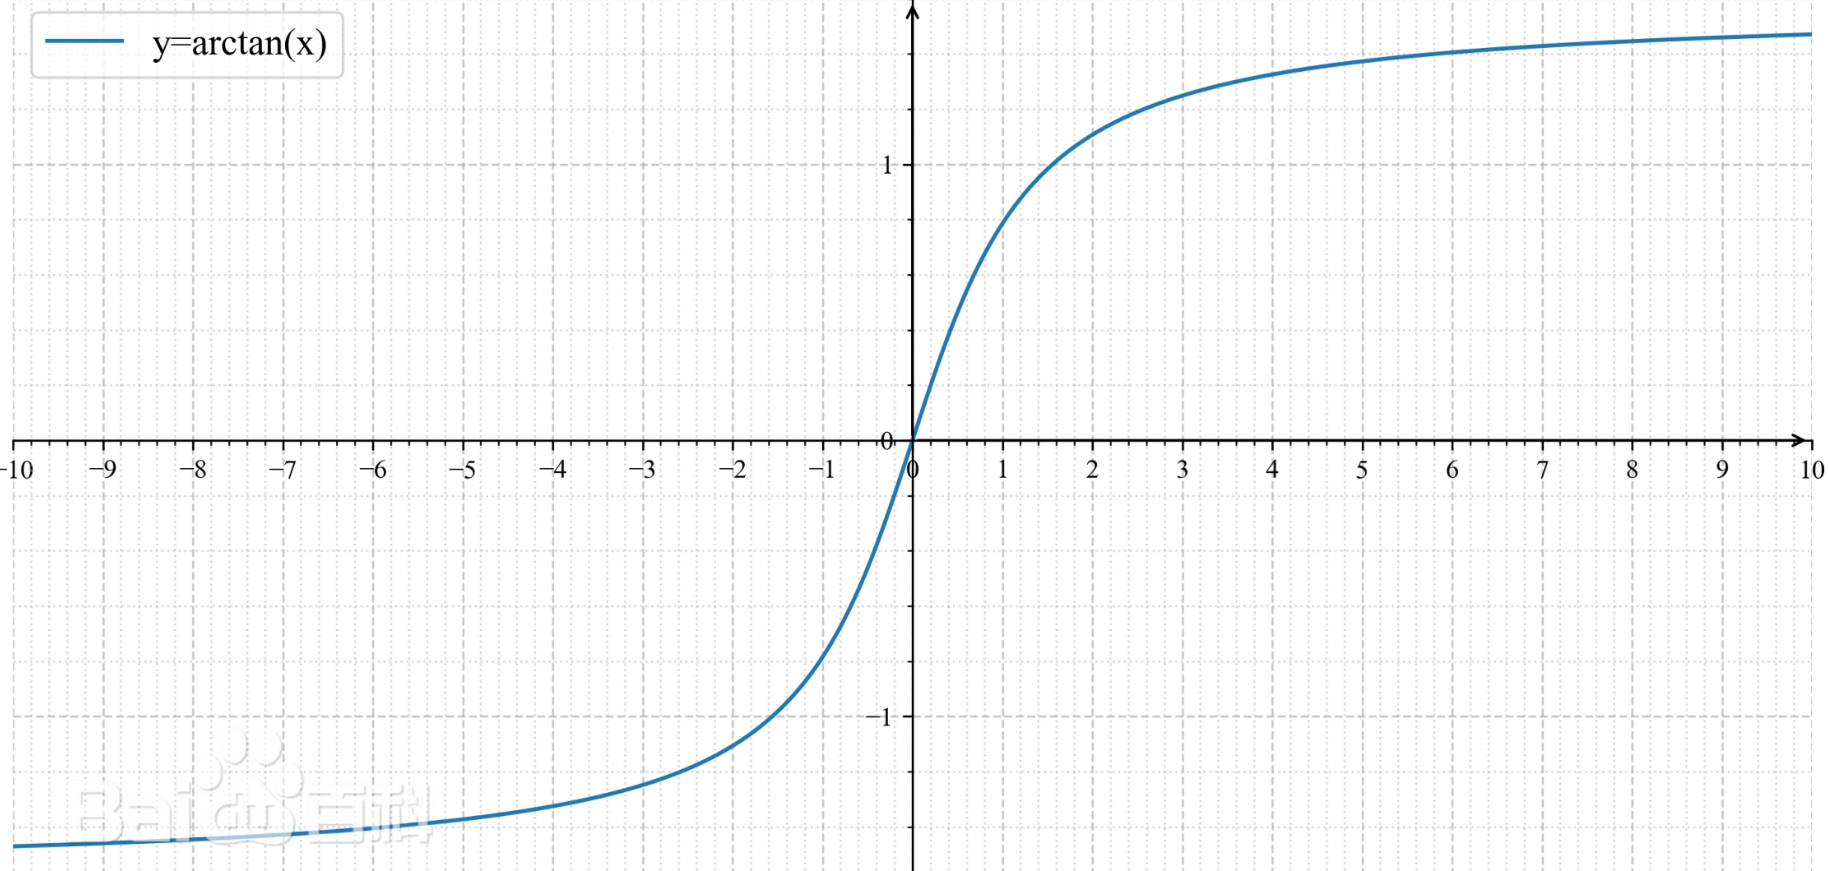
\includegraphics[width=0.8\textwidth]{arctan.png}   
    \caption{The shape of $g(x) = \arctan{x}$}
    \label{fig:arctan}
\end{figure}

The derivative of $g(x)$ is $g'(x) = \cfrac{1}{1+x^2}$ , and we have $|g'(x)| < 1$ for all $x \in (-\cfrac{\pi}{2},\cfrac{\pi}{2})$ except $x = 0$.
But if $x_n = 0$, then the sequence always equals to $0$, which is convergent.

Therefore, according to \textbf{Theorem 1.40}, the iteration converge at last.

\section*{VI.}
$x_1 = \cfrac{1}{p} \in (0,1)$, and $x_{n+1} = \cfrac{1}{p + x_n}$. It's easy to deduce that for all $x_n \in (0,1)$.

The iteration function is $g(x) = \cfrac{1}{p + x}$, so $|g'(x)| = \cfrac{1}{(p + x)^2} < 1, \; x \in (0,1)$.
Therefore, according to \textbf{Theorem 1.40}, the iteration converge at last.

Let $g(x) = x$ and we can solve that the \textbf{fixed point $x = \cfrac{1}{2}(-p + \sqrt{p^2 + 4})$}. (Another solution does not satisfy the conditinal range)

\section*{VII.}
Firstly, we cannot use $a_0$ as the lower bound to estimate the error, because the range contains $0$. So \textbf{the inequality is not valid. }

Also, the original inequality in problem II is not effective under this circumstance, because if the real root $r$ getting really close to $0$,
even though the absolute error $|x_n - \alpha|$ can be really small, but the relative error may still be really huge. Therefore, the relative error is not an appropriate measure either.

We have to use the absolute error in this situation. Base on problem II, the supremum of the distance between the root and the midpoint is $\cfrac{1}{2}h_{n} = (\cfrac{1}{2})^{n+1}(b_0 - a_0)$.

So we have 
\[
\epsilon \geqslant (\cfrac{1}{2})^{n+1}(b_0 - a_0)
\]
for the given error $\epsilon$ at the $n^{th}$ step.
Simplify it and we have
\[
n \geqslant \cfrac{\log (b_0-a_0) - \log \epsilon}{\log 2} - 1
\]

\section*{VIII.}
\subsection*{VIII-a}
The points will converge more rapidly.

From the \textbf{Theorem 1.15}, the convergence rate can be higher than 2 in the case of $f''(\alpha) = 0$.
If the order can be higher, the rate may be higher, too.

\subsection*{VIII-b}
The problem equals to prove $\lim_{n \rightarrow \infty} \cfrac{\alpha - x_{n+1}}{(\alpha - x_n)^2} = c > 0$.

(I racked my brains but still cannot totally prove it, maybe I think it can imitate the proof of Therorem 1.15 based on Taylor Expansion.
Expand the $f(x)$ at the point $x_n$, 
\begin{align*}
f(x) &= f(x_n) + f'(x_n)(x - x_n) + \frac{f''(x_n)}{2}(x - x_n)^2 \\
&\quad + \frac{f^{(3)}(x_n)}{6}(x - x_n)^3 + \cdots + \frac{f^{(k)}(x_n)}{k!}(x - x_n)^k + \mathcal{O}((x - x_n)^{k+1})
\end{align*}
\begin{align*}
f'(x) &= f'(x_n) + f''(x_n)(x - x_n) + \frac{f^{(3)}(x_n)}{2}(x - x_n)^2 + \cdots + \\
&\frac{f^{(k)}(x_n)}{(k-1)!}(x - x_n)^{k-1} + \mathcal{O}((x - x_n)^{k})
\end{align*}
\begin{align*}
f^{(k)}(x) &= f^{(k)}(x_n) + \mathcal{O}(x - x_n)
\end{align*}
when $x = \alpha$, because $\forall i<k,\; f^{(i)}(\alpha)=0$)


\printbibliography

\end{document}